\section{Biblioteca Digital C3-2013-2 CC-CSSJ}

Considere una biblioteca digital (virtual) cuya información se encuentra contenida en 3 archivos:

Cada línea del archivo \texttt{libros.dat} posee la siguiente estructura: id\_libro,titulo,autor,año publicación y el estante en que se ubica físicamente el libro. Suponga que sólo existe una copia por libro.

\begin{figure}[h]
    \centering
    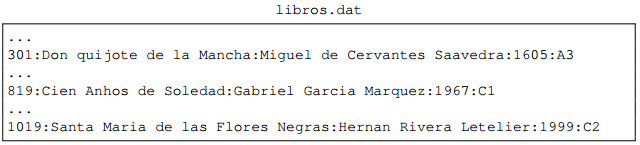
\includegraphics{Imagenes/libros.png}
\end{figure}

Cada línea del archivo \texttt{palabras\_en\_libros.dat} posee la siguiente estructura: palabra: y un listado de \texttt{id\_libro}, en donde aparece la palabra, separado por comas. Suponga que este último listado se encuentra ordenado alfabéticamente.

Finalmente cada línea del archivo \texttt{estado\_libros.dat} posee la siguiente estructura: el \texttt{id\_libro} y su estado ('\texttt{P}' en caso de estar prestado y '\texttt{D}' en caso de estar disponible para préstamo).
Suponga que los identificadores se encuentran ordenados ascendentemente.

\begin{figure}[h]
    \centering
    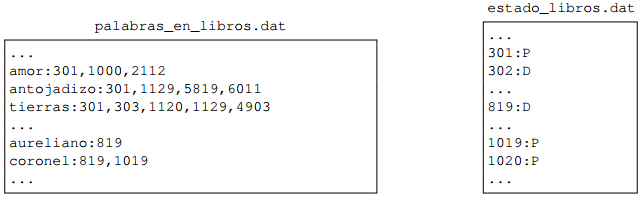
\includegraphics{Imagenes/foto2.png}
\end{figure}

\paragraph{Importante:} Los archivos son en extremo grandes, por lo tanto no es posible almacenar su contenido completo en estructuras estilo diccionario, lista u otros.

Utilizando los archivos presentados se requiere incorporar 3 funcionalidades al sistema de administración de la biblioteca, las que se resumen en 3 subprogramas:

\begin{itemize}
    \item[a)] Construir la función \texttt{buscar(frase)}, que reciba como parámetro un string, que puede estar compuesto por varias palabras separadas por espacio. Esta función debe retornar una lista con la información de los libros que contienen \textbf{por lo menos una} de las palabras
    \begin{lstlisting}[style=consola]
>>> buscar('Coronel Aureliano')
[('Cien Anhos de Soledad', 'Gabriel Garcia Marquez', '1967', 'C1'), 
('Santa Maria las Flores Negras', 'Hernan Rivera Letelier', '1999', 'C2')]
    \end{lstlisting}
    
    \item[b)] Construir la función \texttt{buscar\_disponibles(frase)} que reciba como parámetro un string como el del ejemplo anterior. Esta función debe retornar sólo los libros que se encuentren disponibles.
    \begin{lstlisting}[style=consola]
>>> buscar_disponibles('Coronel Aureliano')
[('Cien Anhos de Soledad', 'Gabriel Garcia Marquez', '1967', 'C1')]    
    \end{lstlisting}
    
    \item[c)] Construir la función \texttt{resevar\_libro(libro)} que reciba como parámetro un entero correspondiente al \texttt{id\_libro}. Esta función debe actualizar el estado del libro en el archivo \texttt{estado\_libros.dat} a '\texttt{P}'
    \begin{lstlisting}[style=consola]
>>> reservar_libro(302)
>>> 
    \end{lstlisting}
\end{itemize}